\subsection{Transportation}
\begin{frame}
\frametitle{Fuel demand}
\begin{columns}
    \column[t]{5cm}
	\begin{figure}[htbp!]
		\begin{center}
			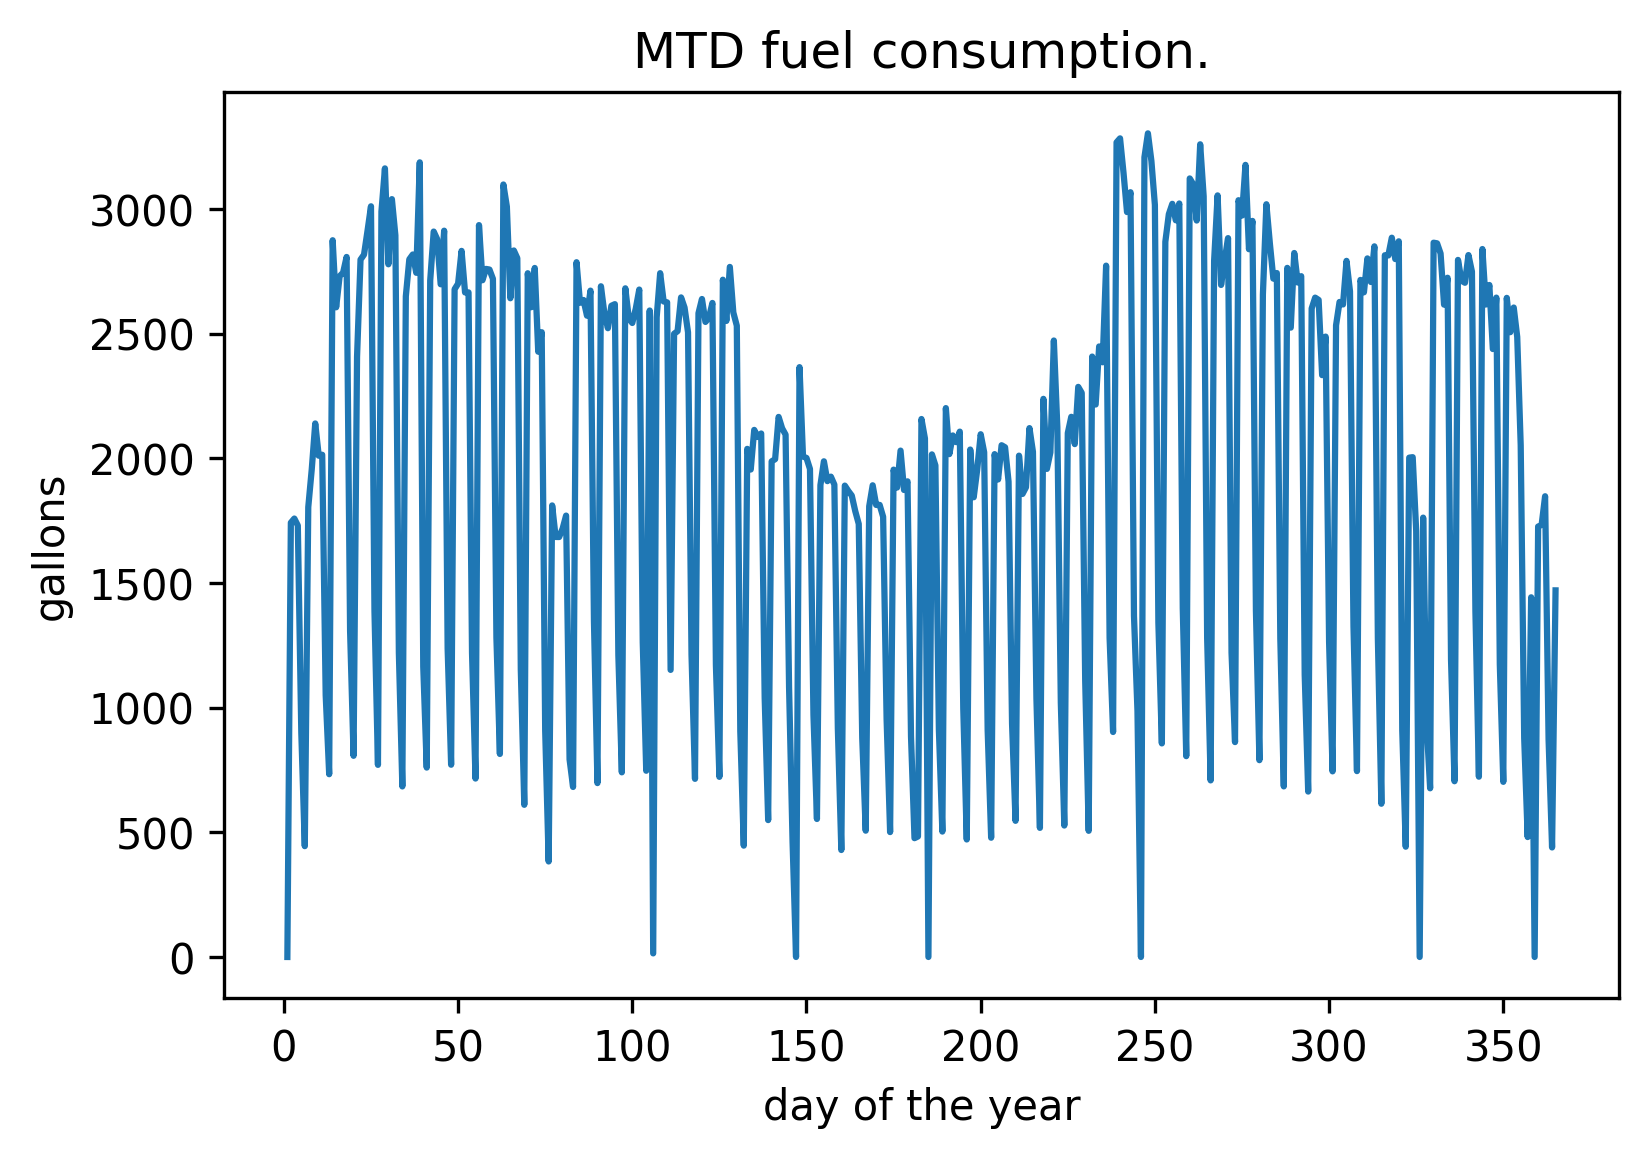
\includegraphics[height=3.5cm]{images/mtd2}
		\end{center}
		\caption{MTD fuel consumption.}
	\end{figure}

	\column[t]{5cm}
	\begin{figure}[htbp!]
		\begin{center}
			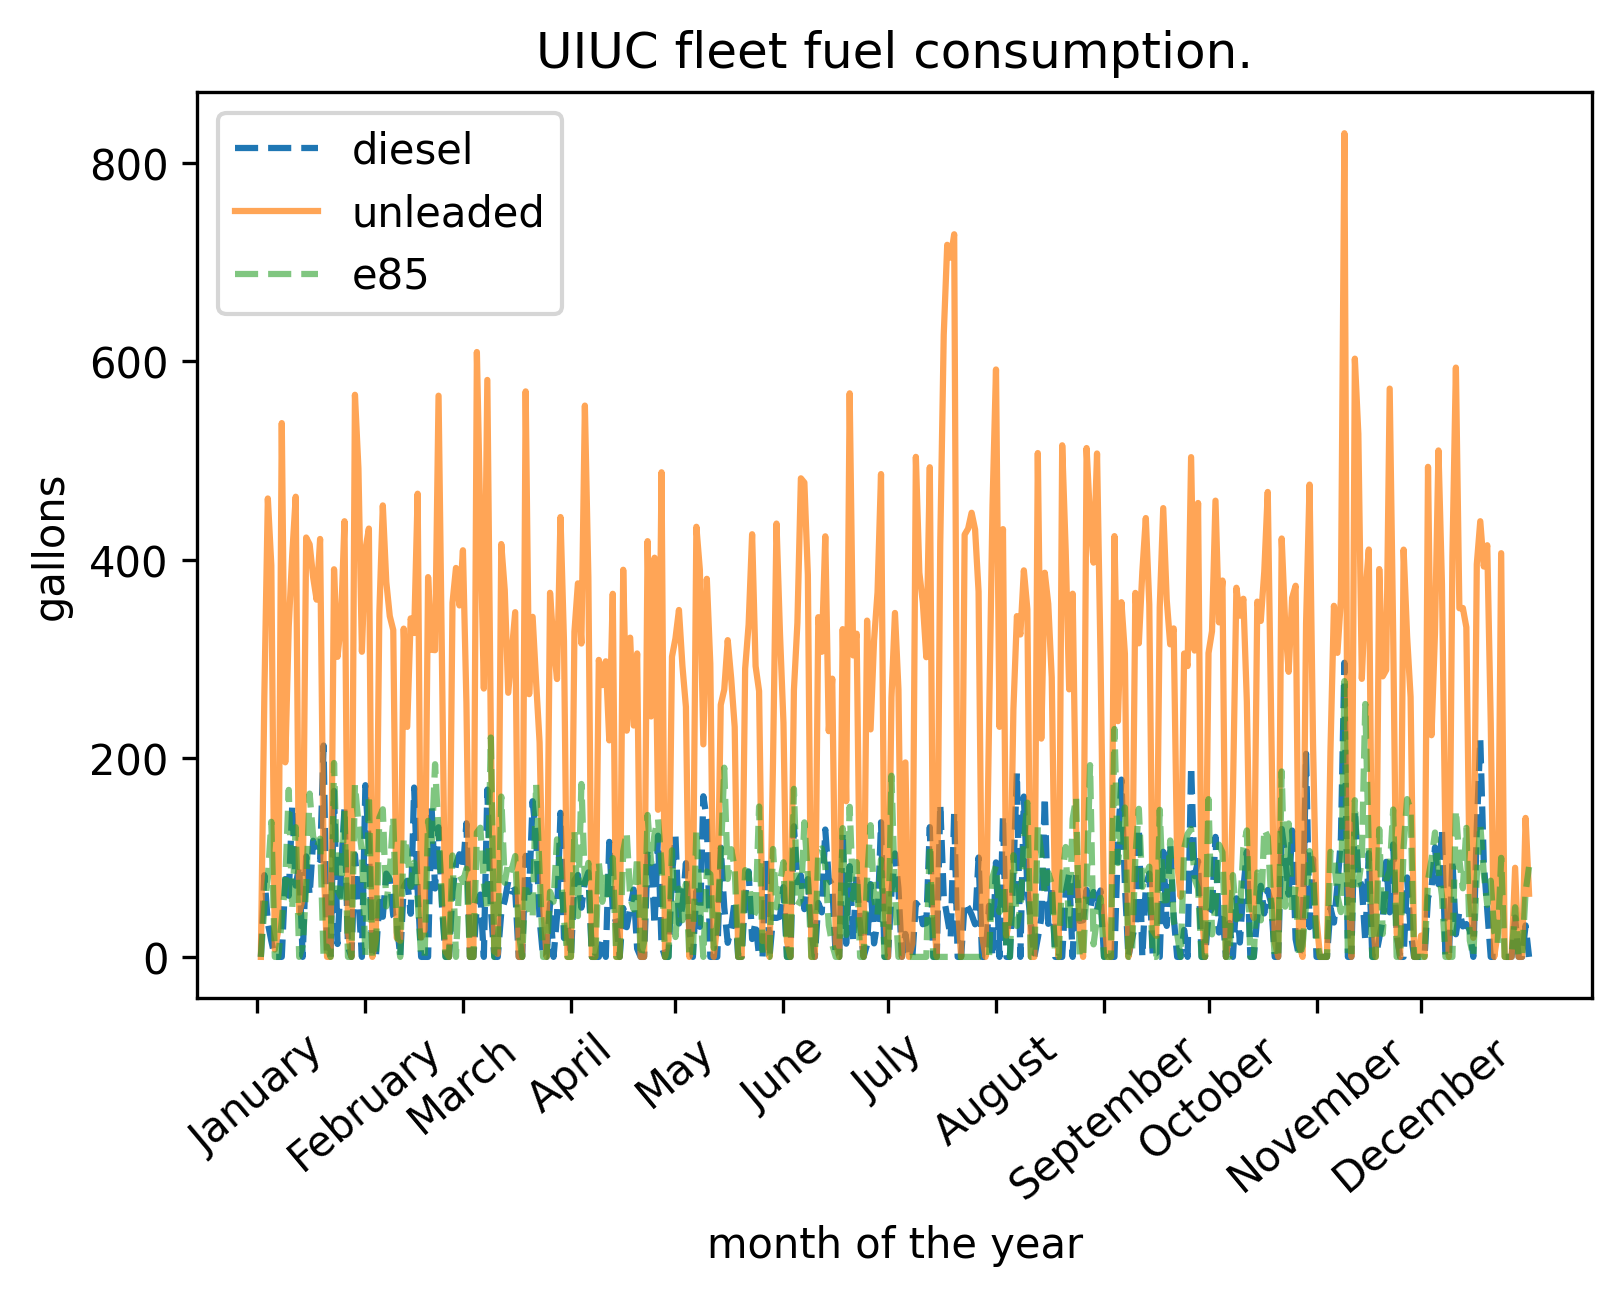
\includegraphics[height=3.5cm]{images/uiuc}
		\end{center}
		\caption{UIUC fleet fuel consumption.}
	\end{figure}
\end{columns}
\end{frame}


\begin{frame}
\frametitle{Hydrogen requirement}
\begin{columns}
    \column[t]{5cm}
	\begin{table}[!htb]
		\centering
	    \caption{GGE, DGE, and E85GE.}
		\begin{tabular}{l|l}
		\hline
		                 & Hydrogen \\ \hline
		GGE              & 1 kg     \\
		DGE              & 1.13 kg  \\
		E85GE            & 0.78 kg  \\ \hline
        \end{tabular}
	\end{table}

	\begin{table}[!htb]
		\centering
	    \caption{Hydrogen requirements.}
		\begin{tabular}{l|l}
		\hline
		Total [tonnes/year]  & 943      \\
		Average [kg/day] 	 & 2584     \\
		Average [kg/h] 		 & 108      \\
		Maximum in one day   & 4440 kg  \\ \hline
        \end{tabular}
	\end{table}

	\column[t]{5cm}
	\begin{figure}[htbp!]
		\begin{center}
			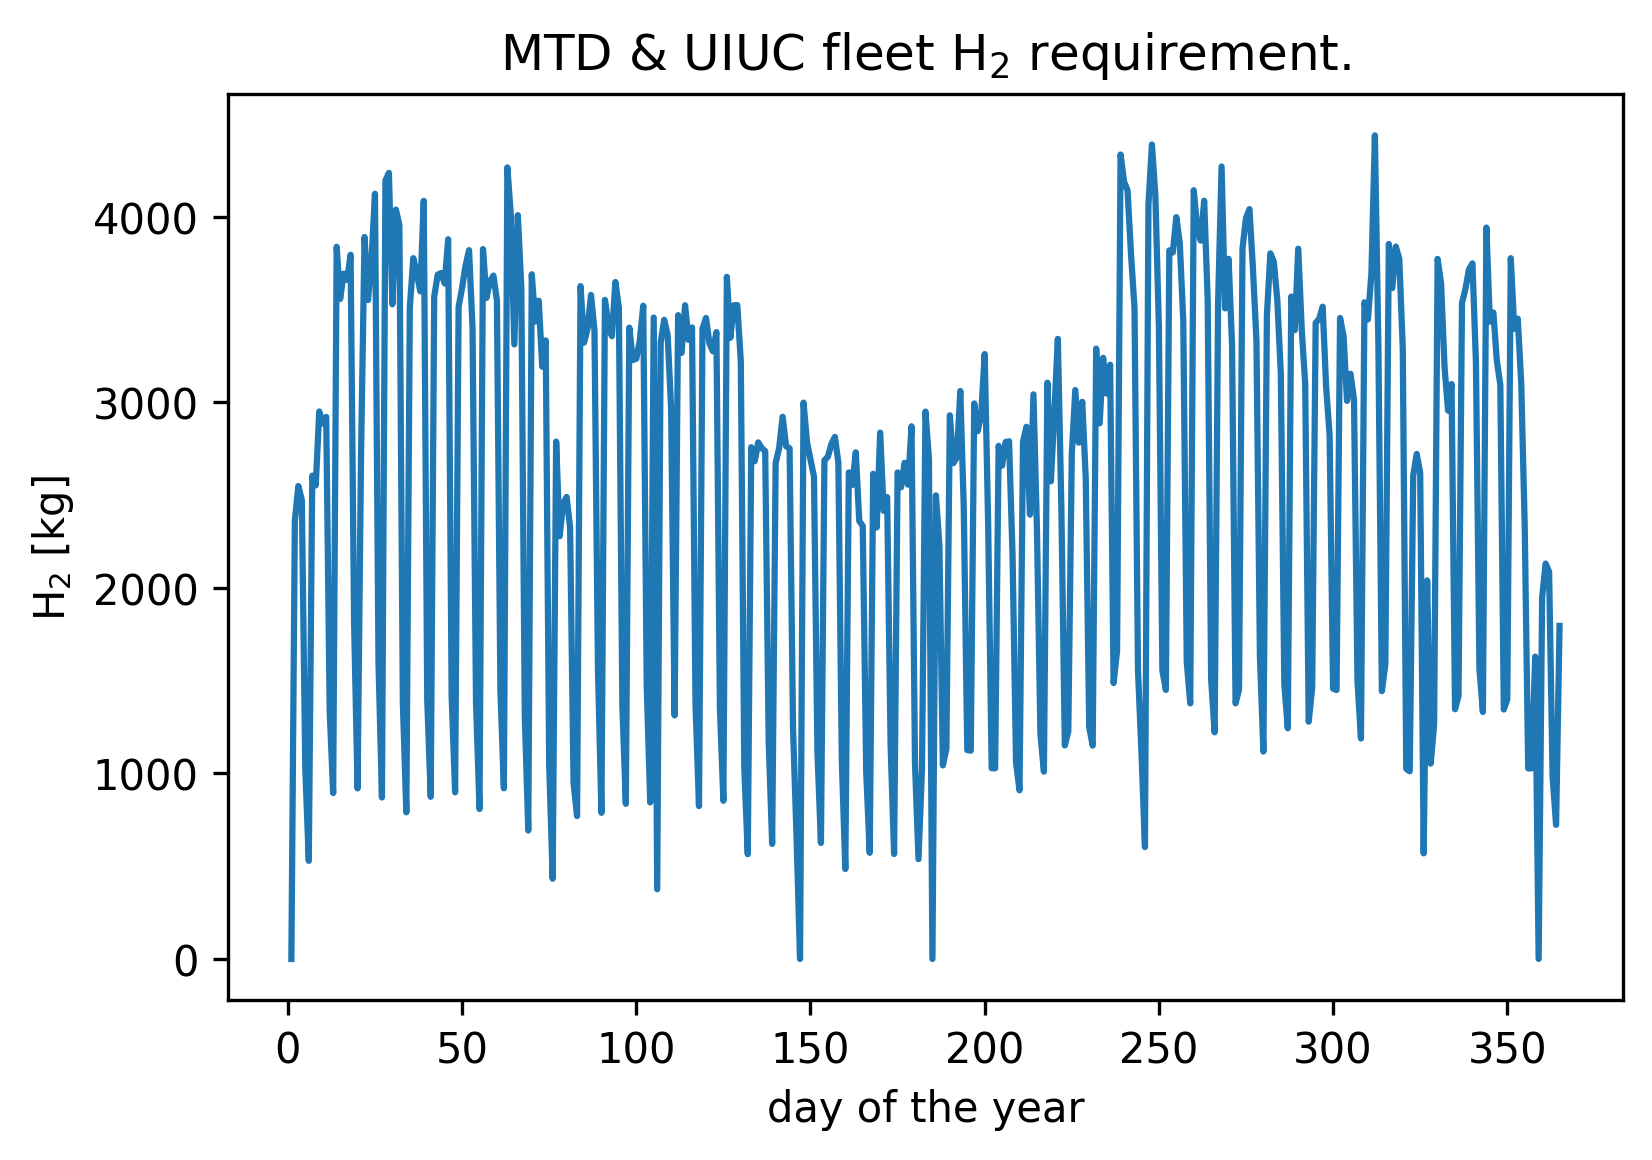
\includegraphics[height=3.5cm]{images/hydro-fleet}
		\end{center}
		\caption{Hydrogen requirement for MTD and UIUC fleets.}
	\end{figure}

\end{columns}
\end{frame}


\begin{frame}
\frametitle{Hydrogen production rate}
\begin{columns}
    \column[t]{4.5cm}
	\begin{table}[!htb]
		\centering
	    \caption{Microreactor designs.}
		\begin{tabular}{l|ll}
		\hline
		Reactor      & P[MW$_{th}$] & T$_o$[$^\circ$C]\\ \hline
		MMR          & 15         & 640             \\
		eVinci       & 5          & 650             \\
		ST-OTTO      & 30         & 750             \\
		U-battery    & 10         & 750             \\
		Starcore     & 36         & 850             \\ \hline
        \end{tabular}
	\end{table}

	\column[t]{5.5cm}
	\begin{figure}[htbp!]
		\begin{center}
			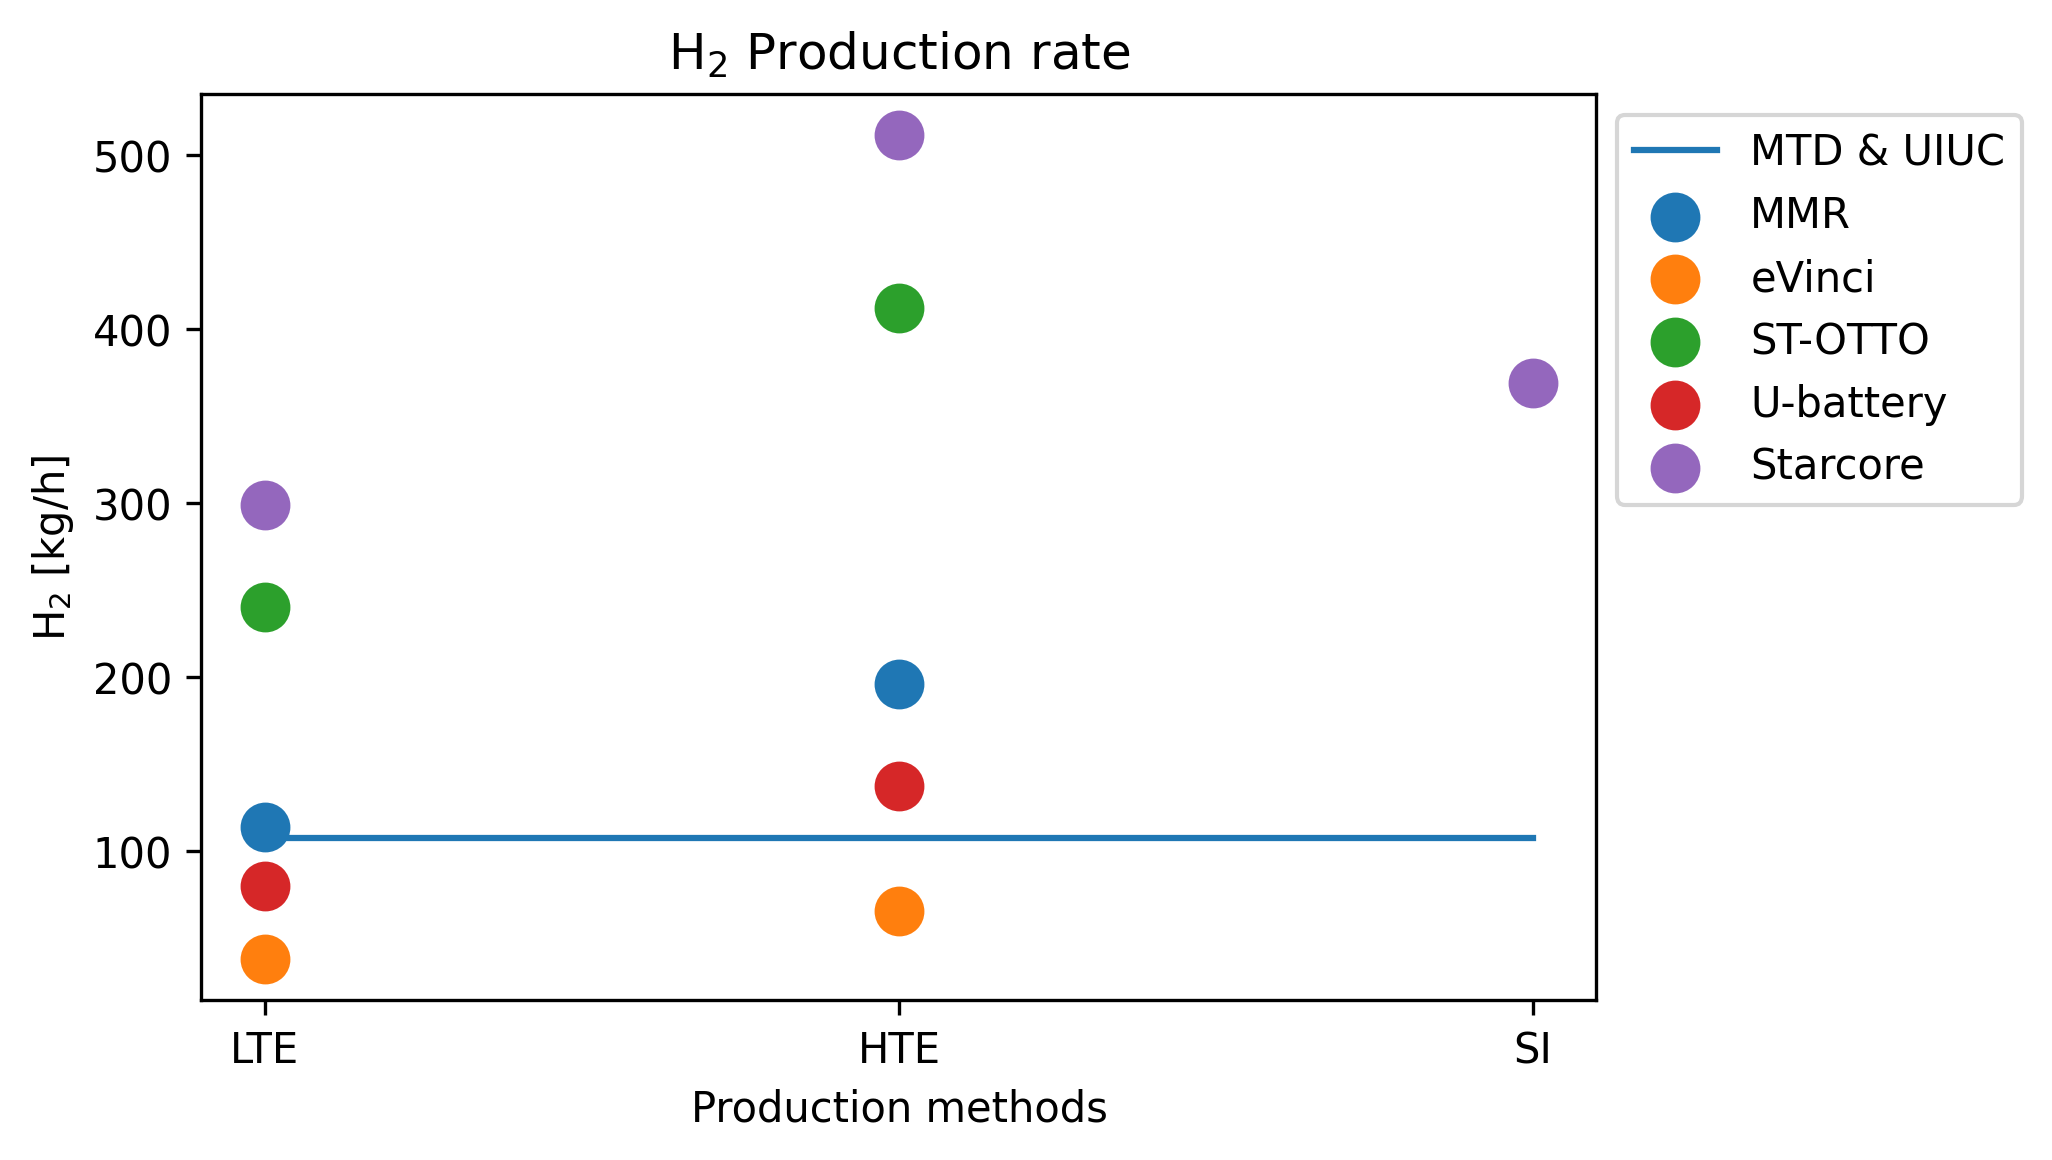
\includegraphics[height=3.5cm]{images/reactors-by-hour1}
		\end{center}
		\caption{Hydrogen production rate by different microreactor designs.}
	\end{figure}

\end{columns}
\end{frame}

\subsection{Energy generation}
\begin{frame}
\frametitle{Net demand prediction}
\begin{columns}
    \column[t]{5cm}
	\begin{figure}[htbp!]
		\begin{center}
			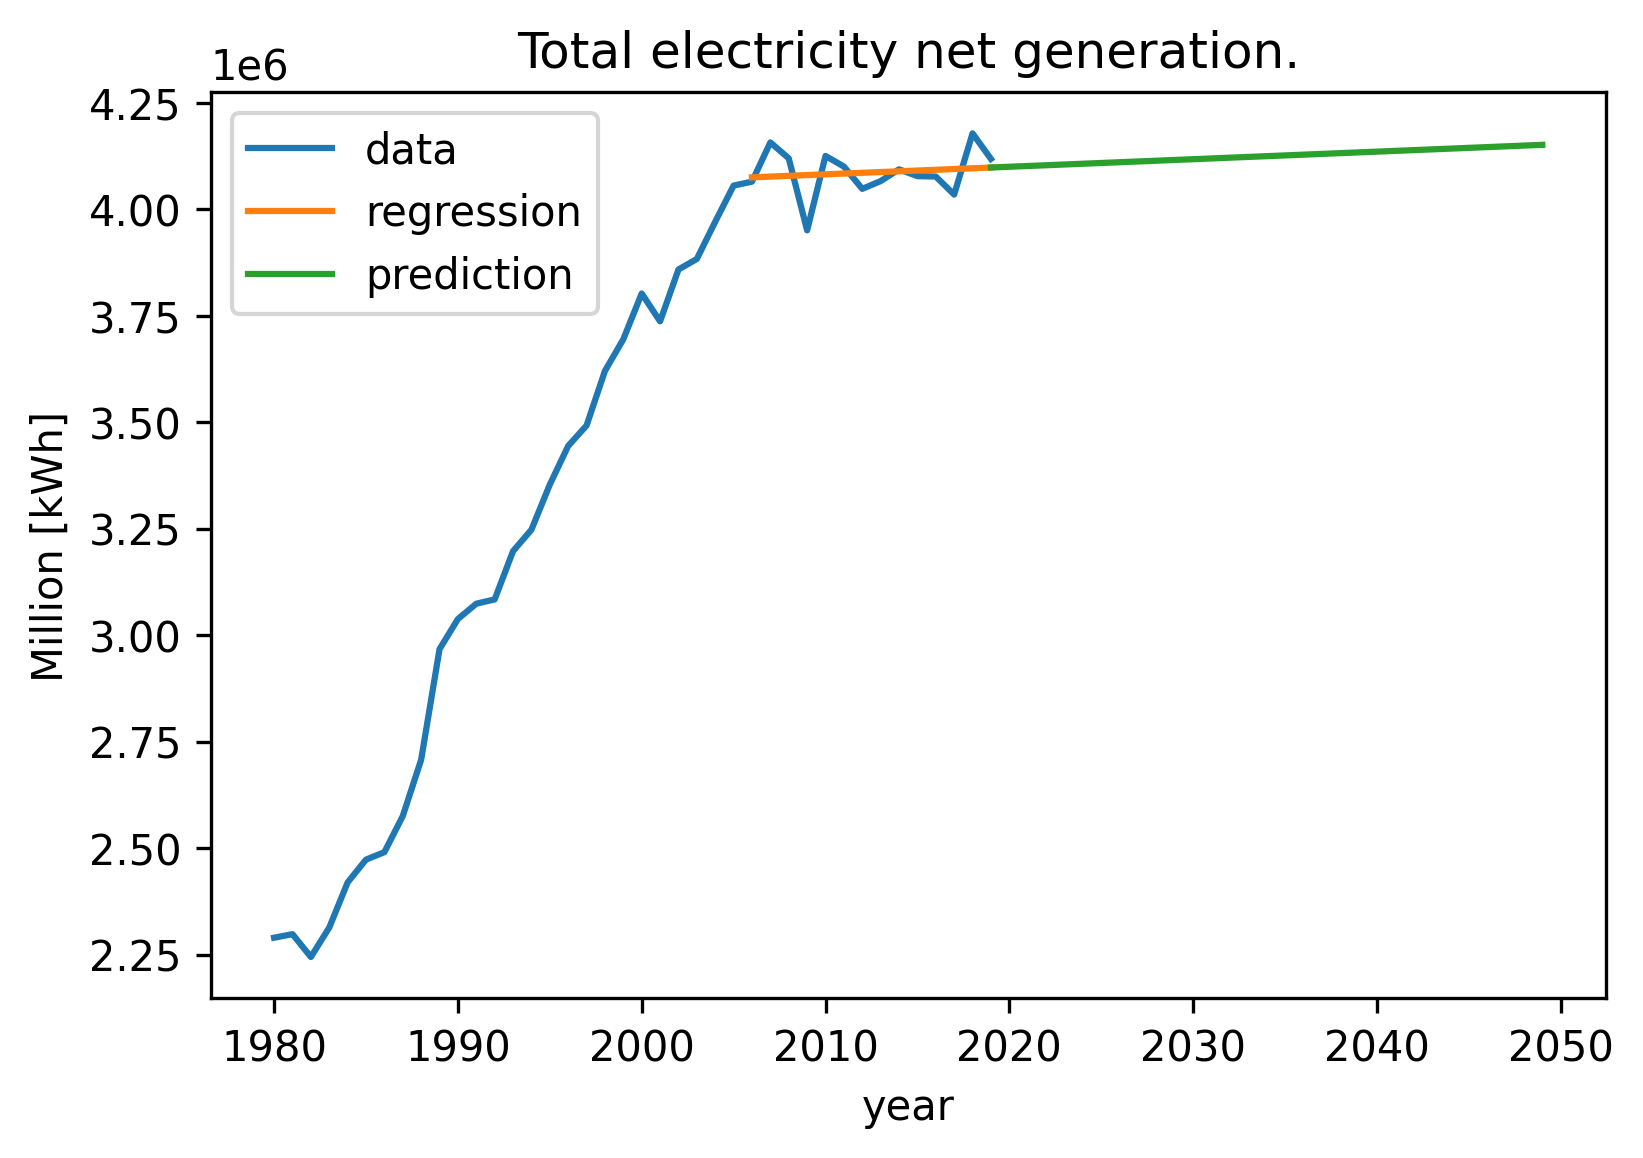
\includegraphics[height=3.3cm]{images/us-prediction1}
		\end{center}
		\caption{Prediction of the total electricity generation in the US for 2050.}
	\end{figure}

    \column[t]{5cm}
	\begin{figure}[htbp!]
		\begin{center}
			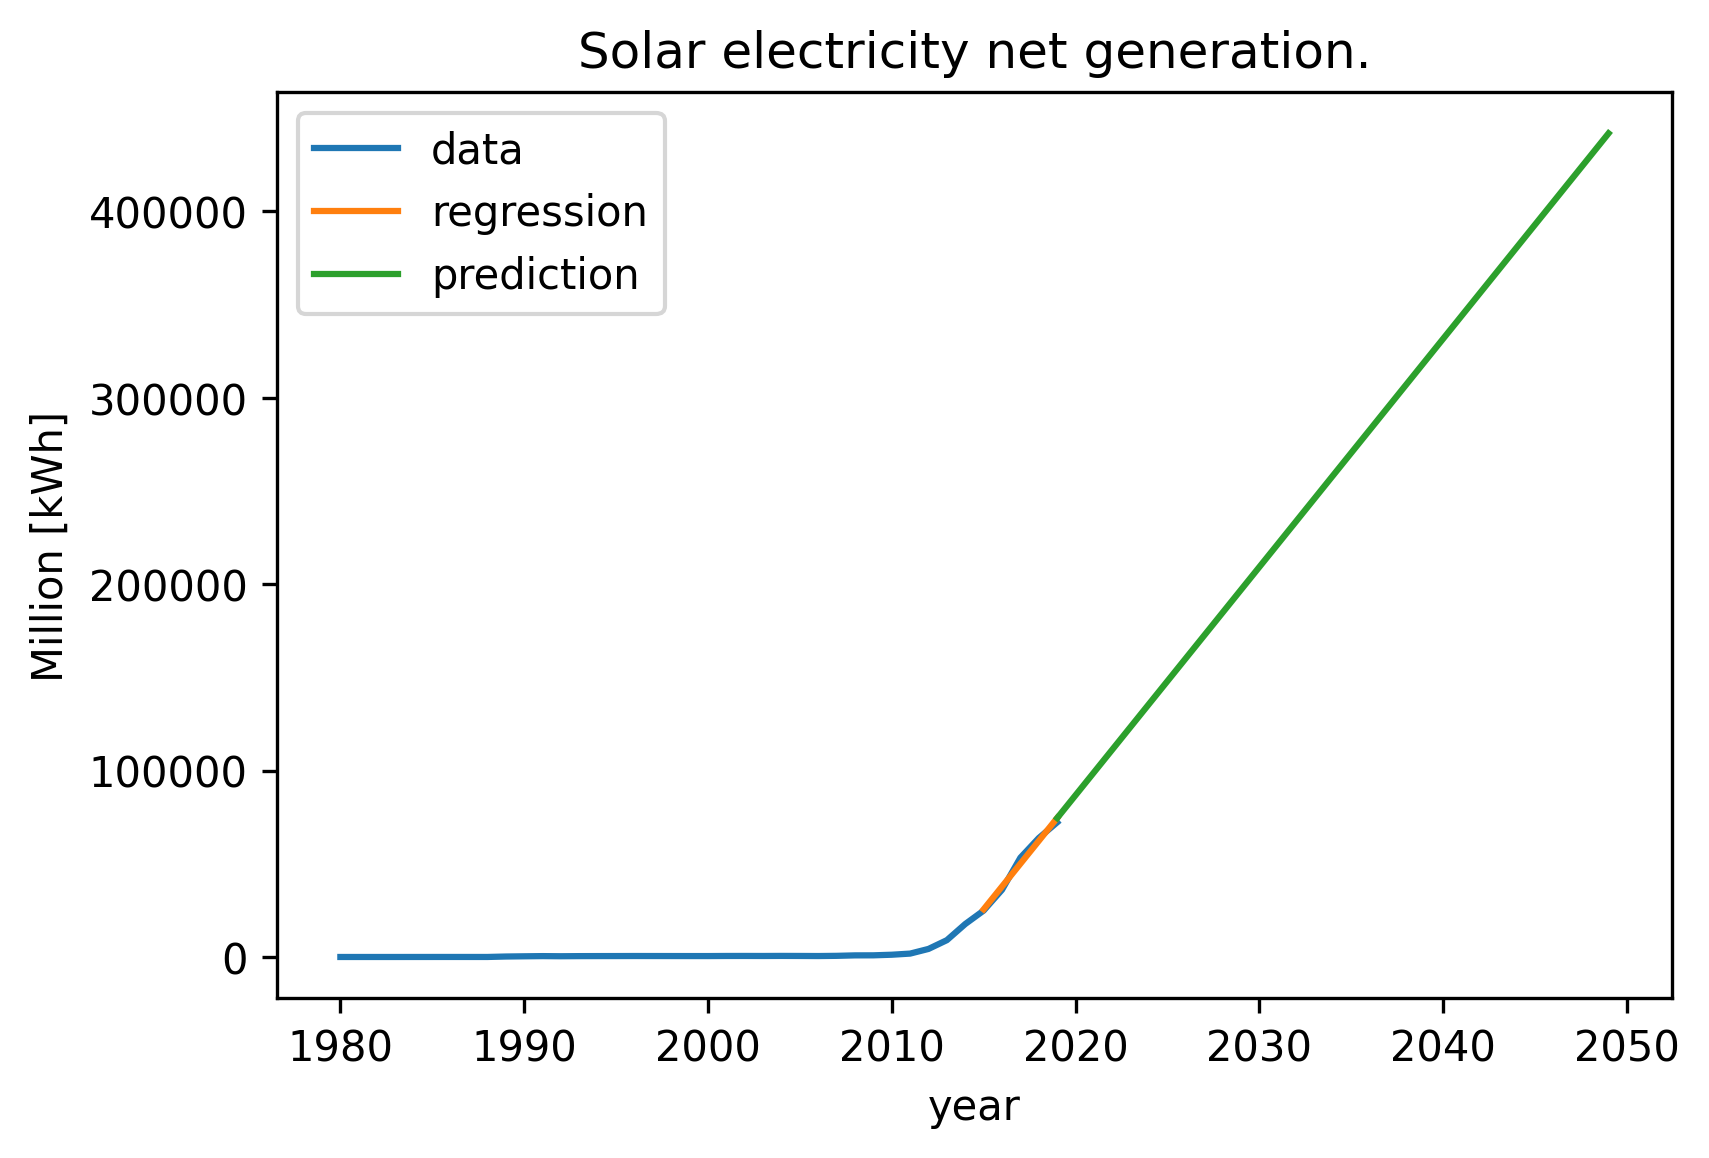
\includegraphics[height=3.3cm]{images/us-prediction2}
		\end{center}
		\caption{Prediction of the solar electricity generation in the US for 2050.}
	\end{figure}
\end{columns}
\end{frame}


\begin{frame}
\frametitle{Duck curve}
\begin{columns}
    \column[t]{4.5cm}
	\begin{figure}[htbp!]
		\begin{center}
			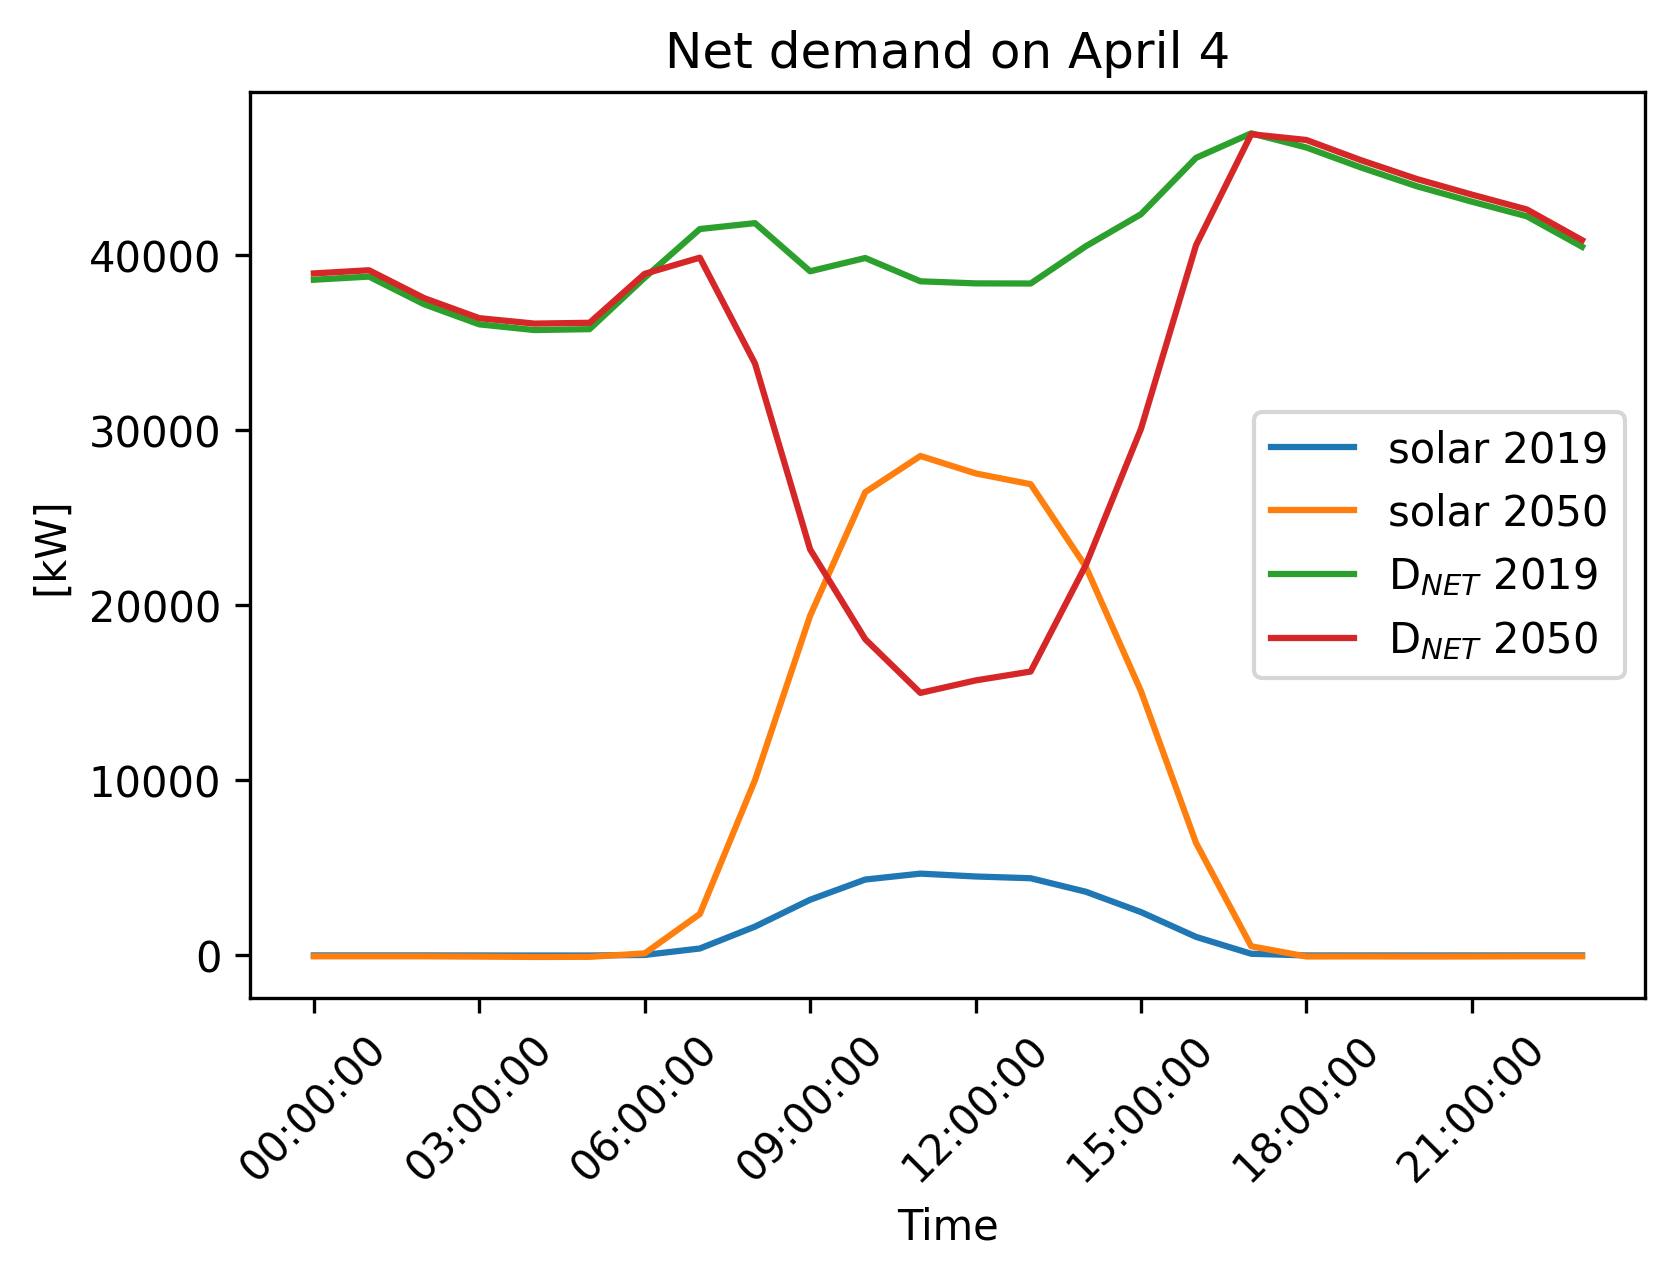
\includegraphics[height=4.0cm]{images/uiuc-duck}
		\end{center}
		\caption{Prediction on UIUC's demand for 2050.}
	\end{figure}

    \column[t]{5.5cm}
    \begin{itemize}
 		\item Spring: solar production is higher, total demand is low.
 		\item Solar generation peaked on April 4, 2019.
 		\item Peak demand is 46.9 MWh at 5 P.M.
 		\item Lowest demand is 15 MWh at 11 A.M.
 		\item Requires an installed capacity of 31.9 MW of dispatchable sources.
 	\end{itemize}

\end{columns}
\end{frame}


\begin{frame}
\frametitle{Over-generation}
\begin{columns}
    \column[t]{5.5cm}
	\begin{figure}[htbp!]
		\begin{center}
			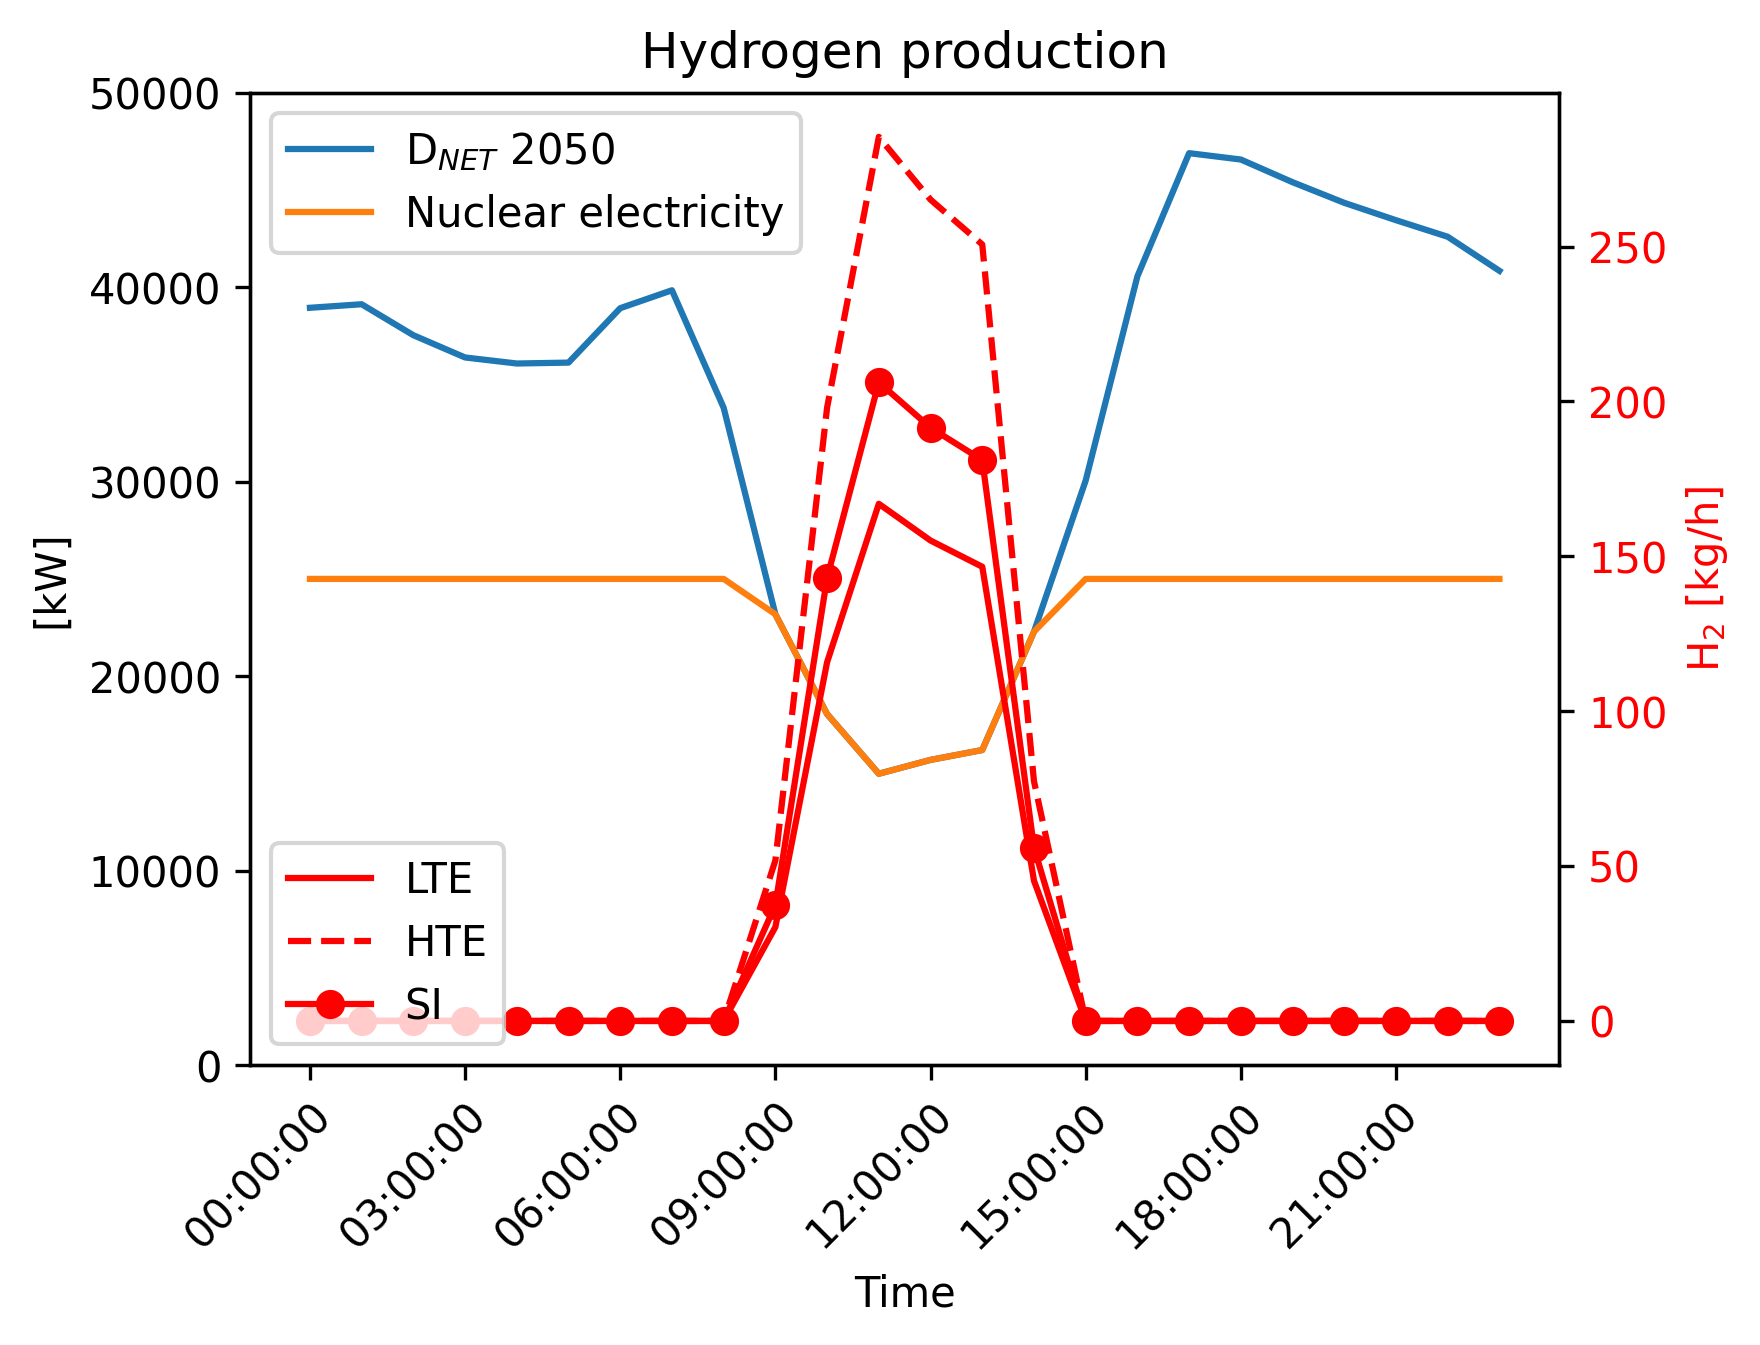
\includegraphics[height=4.4cm]{images/uiuc-hydro2B}
		\end{center}
		\caption{Hydrogen production with the excess of energy.}
	\end{figure}

    \column[t]{4.5cm}
    25 MWe reactor. \vspace{0.2cm}

    LTE:
    \begin{itemize}
 		\item $\eta$=33$\%$.
 		\item 660 kg-H$_2$.
 	\end{itemize}

    HTE:
    \begin{itemize}
 		\item HTGR.
 		\item T$_o$ = 850$^\circ$C.
 		\item $\eta$=49.8$\%$
 		\item 1129 kg-H$_2$.
 	\end{itemize}

    SI:
    \begin{itemize}
 		\item HTGR.
 		\item T$_o$ = 850$^\circ$C.
 		\item $\eta$=49.8$\%$
 		\item 815 kg-H$_2$.
 	\end{itemize}

\end{columns}
\end{frame}

\begin{frame}
\frametitle{Hydrogen for energy storage}
\begin{columns}
    \column[t]{6.5cm}
	\begin{figure}[htbp!]
		\begin{center}
			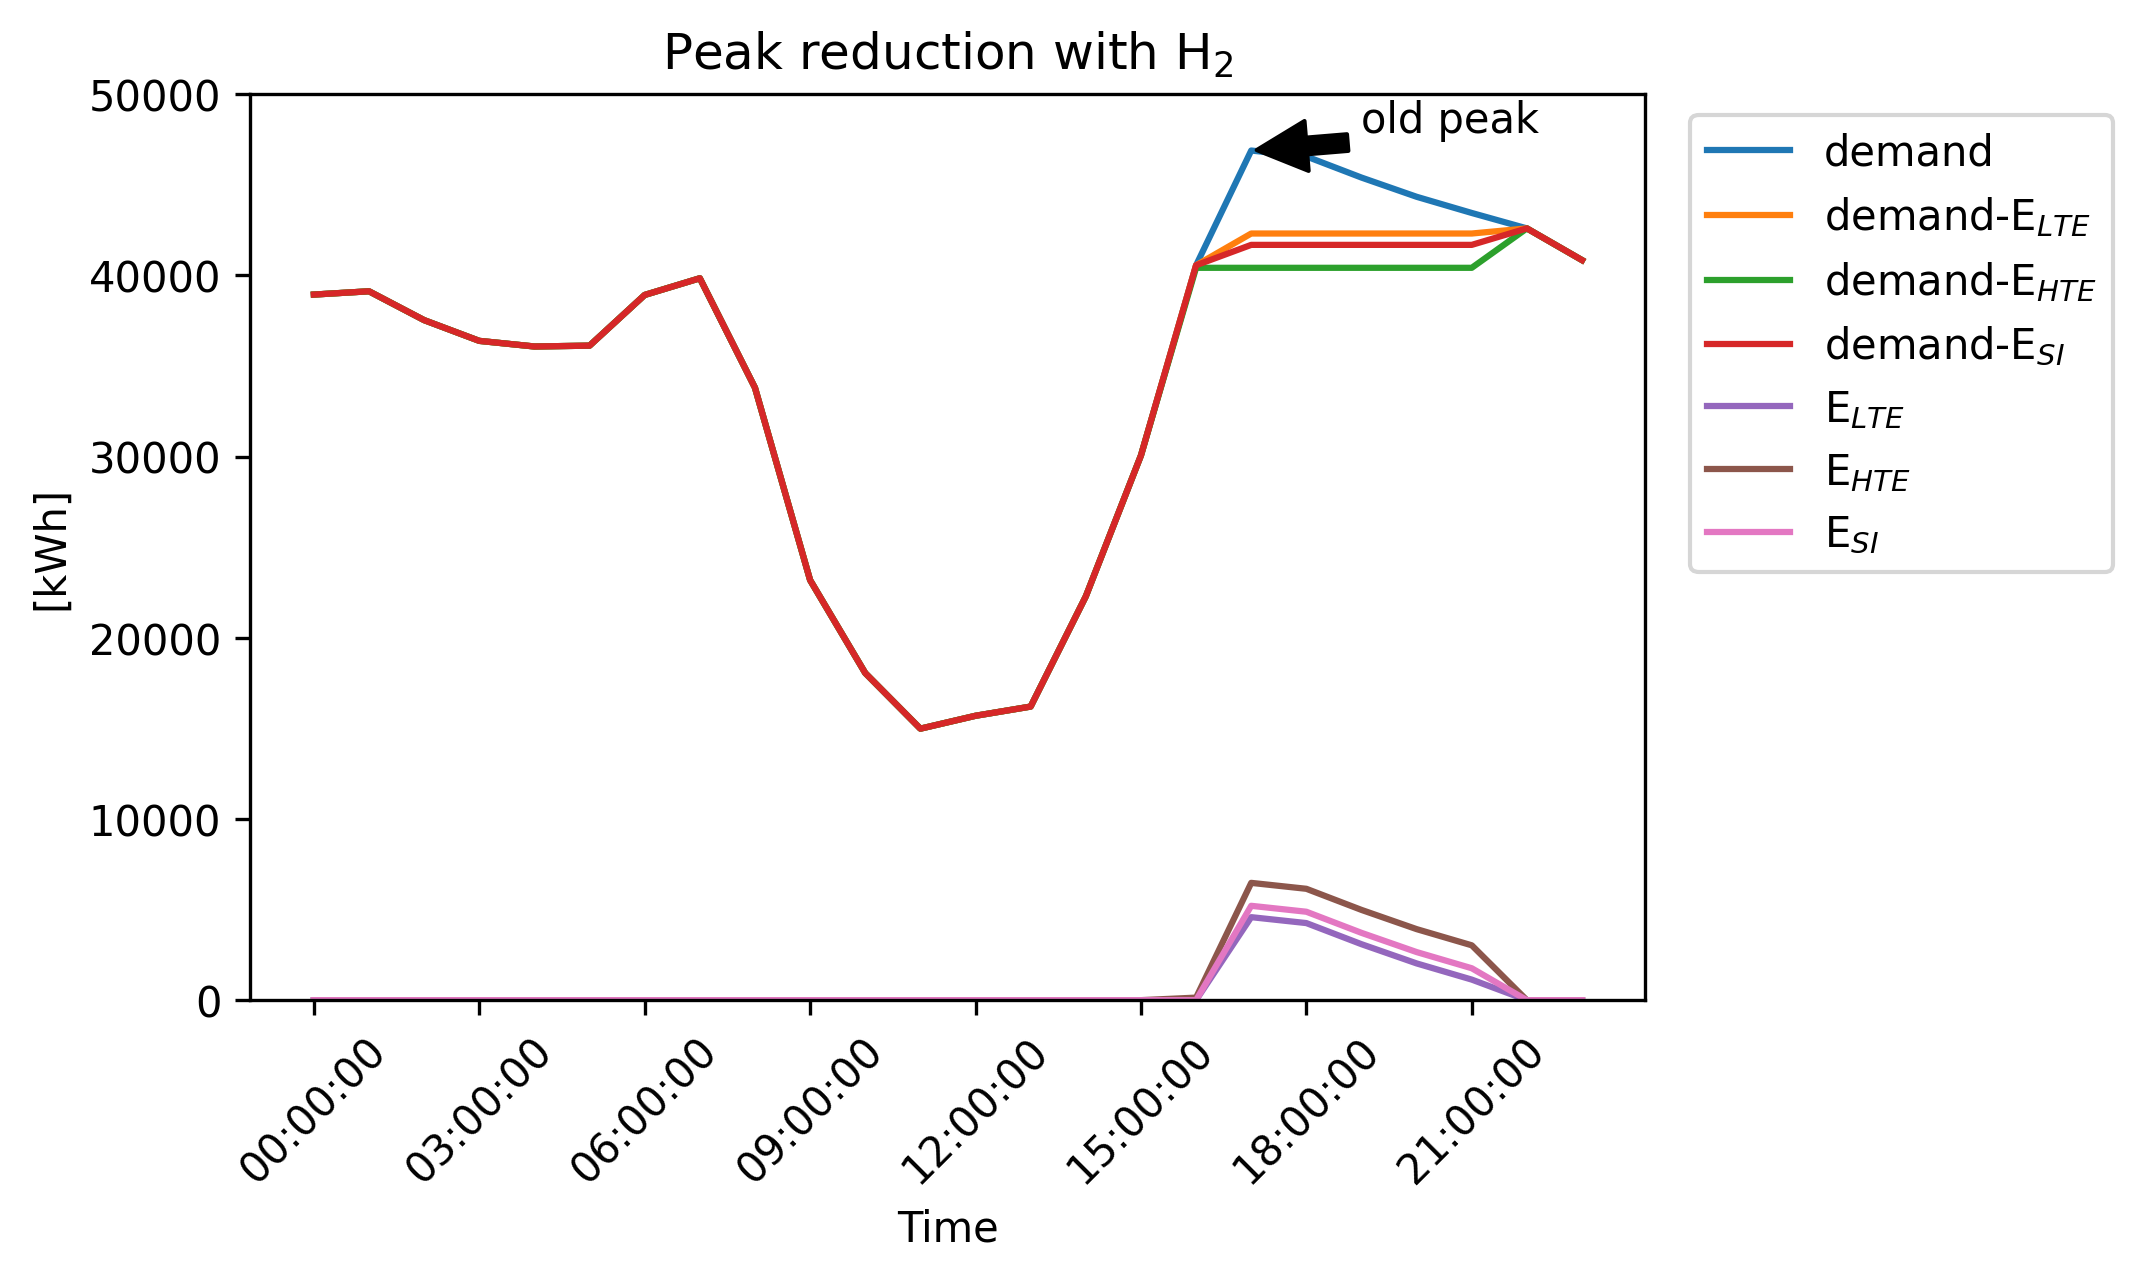
\includegraphics[height=4.2cm]{images/uiuc-hydro3B}
		\end{center}
		\caption{Peak reduction by using the produced H$_2$.}
	\end{figure}

    \column[t]{4.5cm}
    \\
    LTE:
    \begin{itemize}
 		\item 15.9 MWh.
 		\item New peak: 41.9 MWh
 		\item Peak reduction: 5 MWh
 	\end{itemize}

    HTE:
    \begin{itemize}
		\item 27.1 MWh.
		\item New peak: 40.0 MWh
        \item Peak reduction: 6.9 MWh
 	\end{itemize}

    SI:
    \begin{itemize}
		\item 19.6 MWh.
		\item New peak: 41.3 MWh
        \item Peak reduction: 5.6 MWh
 	\end{itemize}

\end{columns}
\end{frame}